\documentclass[a4paper,12pt]{article}           %   A4, pt changes regular font size
\frenchspacing                                  %   Finnish spacing
\usepackage{a4wide}                             %   Less margis
\usepackage[british]{babel}                     %   Edit this to match your language, e.g., finnish
\usepackage{xcolor}                             %   color support
    \definecolor{my_grey}{HTML}{7F7F7F}
\usepackage{icomma}                             %   Better comma in eqs. if used
\usepackage{hyperref}                           %   Clickable URLs
\usepackage{booktabs}                           %   Better tables
\usepackage{siunitx}                            %   Physics unit stuff
\usepackage{listings}                           %   Better tables
\usepackage{graphicx}                           %   Figures work
\usepackage{fontspec}                           %   Better way to handle custom fonts
\usepackage{amsmath}                            %   Basic math
\usepackage{esint}                              %   Various fancy integral symbols
\usepackage[capitalise]{cleveref}               %   \cref better than \ref
    \crefname{section}{Sec.}{Secs.}             %   Add abbreviation for Sections
\usepackage[position=top]{subfig}
    \captionsetup[subfigure]{position=top, labelfont=bf,textfont=normalfont,singlelinecheck=off,justification=raggedright}
\captionsetup[subfigure]{subrefformat=simple,labelformat=simple,listofformat=subsimple}
\renewcommand\thesubfigure{(\alph{subfigure})}
\usepackage{sectsty}                            %   Edit section titles
    %\allsectionsfont{\normalfont\sffamily}     %   ALL titles use sans-serif
    \sectionfont{\normalfont\sffamily\large\color{my_grey}} 
    \subsectionfont{\normalfont\sffamily\normalsize\color{my_grey}} 
    \subsubsectionfont{\normalfont\sffamily\small\color{my_grey}}
\setsansfont{URW Gothic L}[
    Path = fonts/,
    Extension =.ttf,
    UprightFont = * Regular,
    ItalicFont = * Italic,
    BoldFont = * Bold,
    BoldItalicFont= * Bold Italic]
\setmonofont{Source Code Pro}[
    Path = fonts/,
    Extension =.ttf,
    UprightFont = *-Regular,
    ItalicFont = *-Italic,
    BoldFont = *-Bold,
    BoldItalicFont= *-BoldItalic
]
\setmainfont{AdobeTextPro}[
    Scale = 0.958,
    Path = fonts/,
    Extension =.ttf,
    UprightFont = *-Regular,
    ItalicFont = *-It,
    BoldFont = *-Bold,
    BoldItalicFont= *-BoldIt]
\usepackage[libertine]{newtxmath}               %   Matching math font
\usepackage{fancyhdr}                           %   Nice header and footer header (and/or footer)
    \pagestyle{fancy}                               %   Makes package work
\usepackage[section]{placeins}                  %   Figures stay in declared section
\usepackage{minted}                             %   Beautiful verbatim code
    \usemintedstyle{emacs}                          %   code style
    \setminted{
        frame=lines,
        framesep=2mm,
        baselinestretch=0.9,
        fontsize=\footnotesize,
        linenos,
        breaklines
    }
\usepackage{csquotes}                           %   Correct quotes for babel
\usepackage[backend=biber,
            style=ieee,
            urldate=long,
            maxnames=5,
            dateabbrev=false]{biblatex}         %   Citation style with biblatex
\DeclareSourcemap{                              %   No ISSN for journals
    \maps[datatype=bibtex]{
        \map{
        \step[fieldset=issn, null]
        }
    }
}
\renewbibmacro*{doi+eprint+url}{                %   Print URL iff no doi
    \printfield{doi}
    \newunit\newblock{}
    \iftoggle{bbx:eprint}{
        \usebibmacro{eprint}
    }{}
    \newunit\newblock{}
    \iffieldundef{doi}{
        \usebibmacro{url+urldate}}
        {}
}

\hypersetup{
    pdfauthor={Niko Savola},                    %   Author here
}

\linespread{1.1}
\setlength{\headheight}{15pt}                   %   Suppress height warnings
\addtolength{\topmargin}{-2.4pt}


% Set commonly used math commands here
\newcommand*{\pd}[3][]{\ensuremath{\frac{\partial^{#1} #2}{\partial #3}}}
\newcommand*{\dt}[3][]{\ensuremath{\frac{\textrm{d}^{#1} #2}{\textrm{d} #3}}}
\newcommand{\dbar}{\textrm{d}\hspace*{-0.08em}\bar{}\hspace*{0.1em}}
\newcommand{\de}{\textrm{d}}
\newcommand{\sref}[1]{\textbf{\small\subref{#1}}}
\newcommand{\ve}[1]{\textbf{#1}}
\newcommand{\e}{\mathrm{e}}

\addbibresource{references.bib}
\hypersetup{
    pdftitle={Machine learning with many-body tensor networks | Niko Savola},
}
%   header
\lhead{\textsf{Special exercise}}
\chead{\textsf{PHYS-E0421 - Solid-State Physics}}
\rhead{\textsf{Niko Savola \textbf{653732}}}
%   footer
\lfoot{}
\cfoot{}
\rfoot{\thepage}


\usepackage[braket, qm]{qcircuit}  % Qiskit output


\begin{document}

\begin{titlepage}
    {\sffamily
    \noindent
    \fontsize{12}{14}\selectfont
    Aalto University \newline
    School of Science \newline
    Department of Applied Physics

    \vspace{40mm}

    \noindent
    \fontsize{14}{16}\selectfont
    \emph{Niko Savola}

    \vspace{10mm}

    \noindent
    \fontsize{18}{22}\selectfont
    \textbf{Machine learning with many-body tensor networks}\\

    \fontsize{12}{14}\selectfont
    \noindent
    Submitted for approval: \today

    \vspace{70mm}

    \noindent
    Special exercise \\[4mm]
    PHYS-E0421 \textendash{} Solid-State Physics \\[4mm]
    } % end of \sffamily

\end{titlepage}
\newpage


\section{Introduction}

TODO review paragraph.
https://youtu.be/q8UTwdjS95k

Central to these developments are
tensor-network representations of many-body quantum states.
These are successful variational families of many-body wave
functions, naturally emerging from low-entanglement representations of quantum states (Verstraete, Murg, and Cirac,
2008). T

\section{Theory}

\subsection{Tensor networks}

TODO notation from https://arxiv.org/pdf/1905.01330.pdf

\subsection{Modelling many-body physics}

todo work as Ansätze


\subsection{Numerical implementation}


https://quimb.readthedocs.io/en/latest/examples/ex_tn_train_circuit.html


\cite{Roberts2019}


\section{Results}

todo


\begin{figure}[htb]
    \centering

    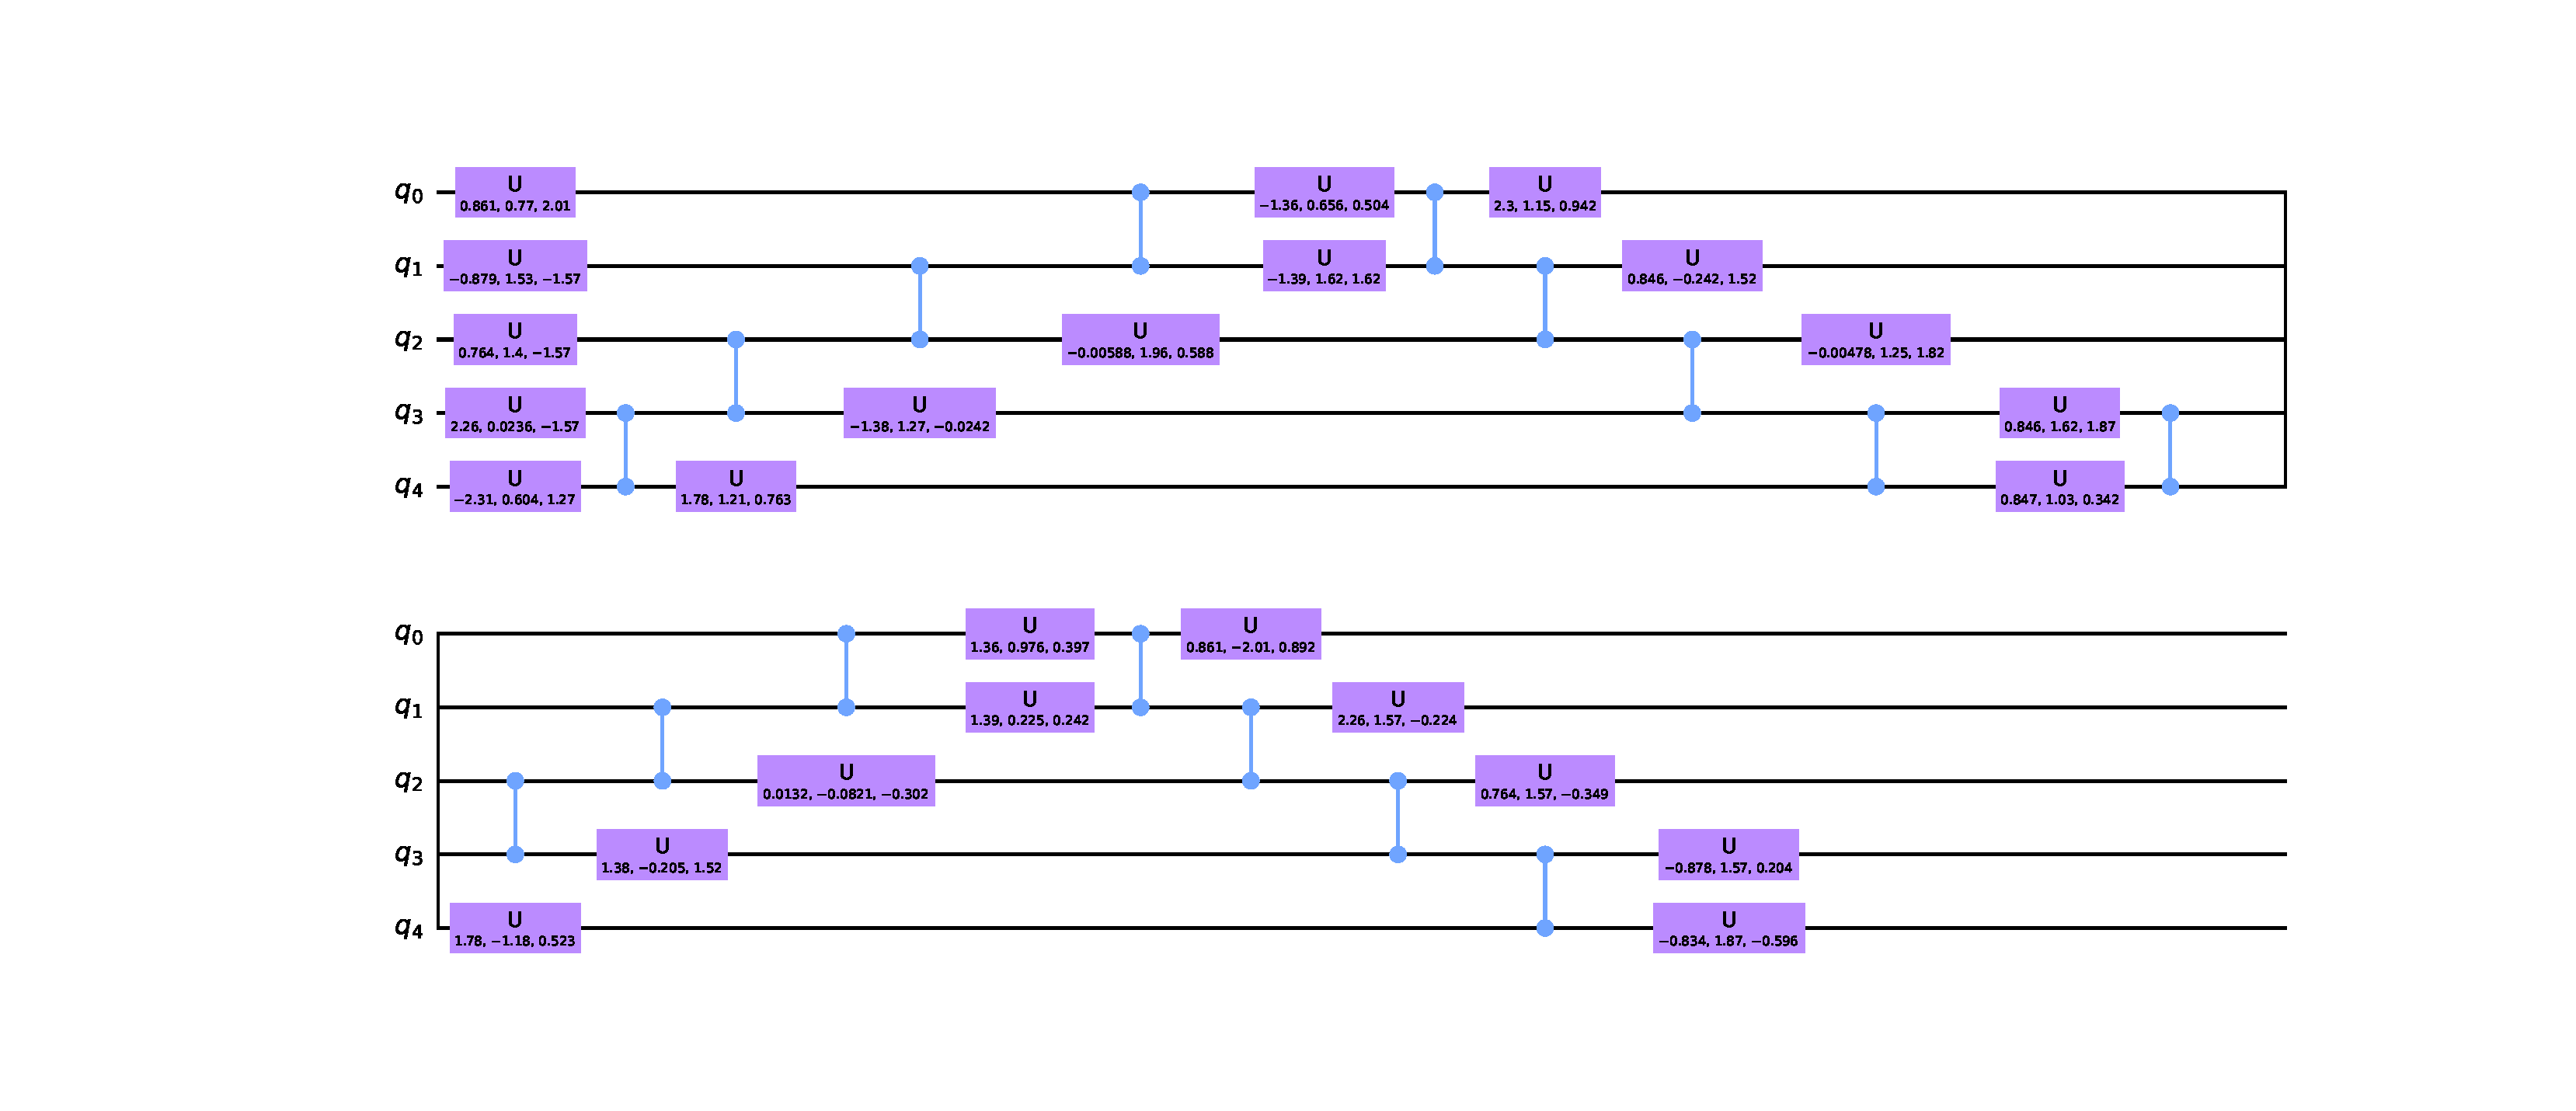
\includegraphics[width=0.97\textwidth]{figures/ansatz_circuit.pdf}

    \caption{<caption>}
    \label{fig:qasm_circuit}
\end{figure}


\section{Summary}

Todo





TODO https://github.com/google/TensorNetwork

https://arxiv.org/pdf/1905.01331.pdf

%-------------------
%   Bibliography
%-------------------

\newpage
\pagestyle{plain}
%\setlength\bibitemsep{1.3\itemsep}
%\setlength\bibitemsep{0.1\baselineskip}
\addcontentsline{toc}{section}{Viitteet}
\renewcommand*{\bibfont}{\footnotesize}
\printbibliography{}


\end{document}
